%Class
\documentclass{article}
%Preamble
\usepackage{graphicx}
\usepackage[left=2.5cm, right=2.5cm, top=3cm, bottom=3cm]{geometry}
\usepackage{url}
\usepackage{enumerate}

%Fonts
\usepackage{helvet}
\renewcommand{\familydefault}{\sfdefault}

%Doc
\begin{document}
\title{Bienvenido a MOOGLE!}
\author{Rafael Sánchez Martinez}
\maketitle

\begin{figure}[h]
    
\includegraphics[width=470px]{Assets/moogle.png}
    %\caption{Moogle Search Engine}
\end{figure}

\begin{quote}
1er Proyecto de Programación - MatCom

Curso 2023-24

Grupo: C-122
\end{quote}

\section*{Features}\label{sec:ent}
\begin{itemize}
    \item
  Soporta búsqueda de temas varios.
    \item
  Modo Oscuro y Modo Claro.
    \item
  Relativamente rápido, probado con 30 documentos(\textasciitilde40mb).
    \item
  Capacidad de uso de operadores de Inclusión (`\^{}'), Exclusión(`!') y
  Cercanía(`\textasciitilde{}').
    \item
  Posibilidad de devolver sugerencias, una vez la consulta sea procesada
  y determinada incorrecta o inexistente en el Corpus.
    \item
  Muestras de pequeñas secciones de los documentos donde se haya
  encontrado lo solicitado.
    \item
  Muestra el Puntaje otorgado a cada documento dependiendo de lo
  consultado.
\end{itemize}

\section{Funcionamiento}
\begin{enumerate}
    \item Como comenzar:
        \begin{itemize}
            \item Si usted se encuentra en Linux, ejecutar en la carpeta del proyecto desde una terminal:
        
            \fbox{make dev}

            \item Si usted se encuentra en Windows o MacOS, ejecutar en la carpeta del proyecto desde una terminal: 
            
            \fbox{dotnet watch run --project MoogleServer}
        \end{itemize}
    \item Inicio:
        \begin{enumerate}
            \item En la zona superior derecha elegir los modos(Oscuro, OscuroSólido, ClaroSólido).
            \item El programa inicia en \texttt{``Program.cs''}
            \begin{itemize}
                \item Linea 5 \fbox{Moogle.LetsGetStarted(@"..//Content");}
                \item Esta es la función invocada presente en "Moogle.cs": Linea-13 
                
                \fbox{public static void LetsGetStarted(string path){ corpus = new Corpus(path); }}
            \end{itemize}
            \item 2.1 Aqui se le da paso al motor de busqueda, que tratará de crear el Diccionario "GeneralFiler" que contendrá todas las palabras de los documentos 'MASE Corpus -> Linea 4'
            \item 2.2 Tambien se creará el diccionario casi más relevante del proyecto, "Docs", que almacenará cada documento con sus datos 'MASE Corpus -> Linea 5'
        \end{enumerate}
    \item Corpus:
        \begin{itemize}
            \item 3.1 Se ejecuta el constructor de esta clase:
            \begin{itemize}
                \item 3.1.1 - \fbox{GetInfo()}, esta función extraerá los archivos de la carpeta content y los agregará al GeneralFiler(VocabularioGeneral)
                \item 3.1.2 - \fbox{IDF()}, esta funcion calculará el IDF de las de los documentos, llamando la funcion IDF de la linea 72 de esa misma clase.
                \item 3.1.3 - \fbox{WW()}o Peso de la palabra, esta funcion la uso para guardar el peso de cada palabra en su documento
                    \begin{itemize}
                        \item 3.1.3.1 Aquí se ejecuta la funcion \fbox{Peso()}, perteneciente a la clase 'Data'(Explicada más adelante), pero no hace más que calcular el peso de cada palabra y darle valor modular al documento procesado en cuestión .
                    \end{itemize}
            \end{itemize}
            \item 3.2 En las anteriores funciones se utilizaba la función BuildGeneralFiler, la cual como su nombre indica, se encarga de construir en GeneralFiler(VocabularioGeneral), pero además procesar y desarrollar el diccionario "Docs".
                \begin{itemize}
                    \item 3.2.1 Aqui creo el objeto data Data data = new Data(); y el conteo que indica cada palabra \fbox{int count = 0}
                \end{itemize}
            \item Esta zona del código fue un descubrimiento excepcional, estoy orgulloso de ello, horas en la página de Microsoft(no es broma)
            
            \begin{figure}
                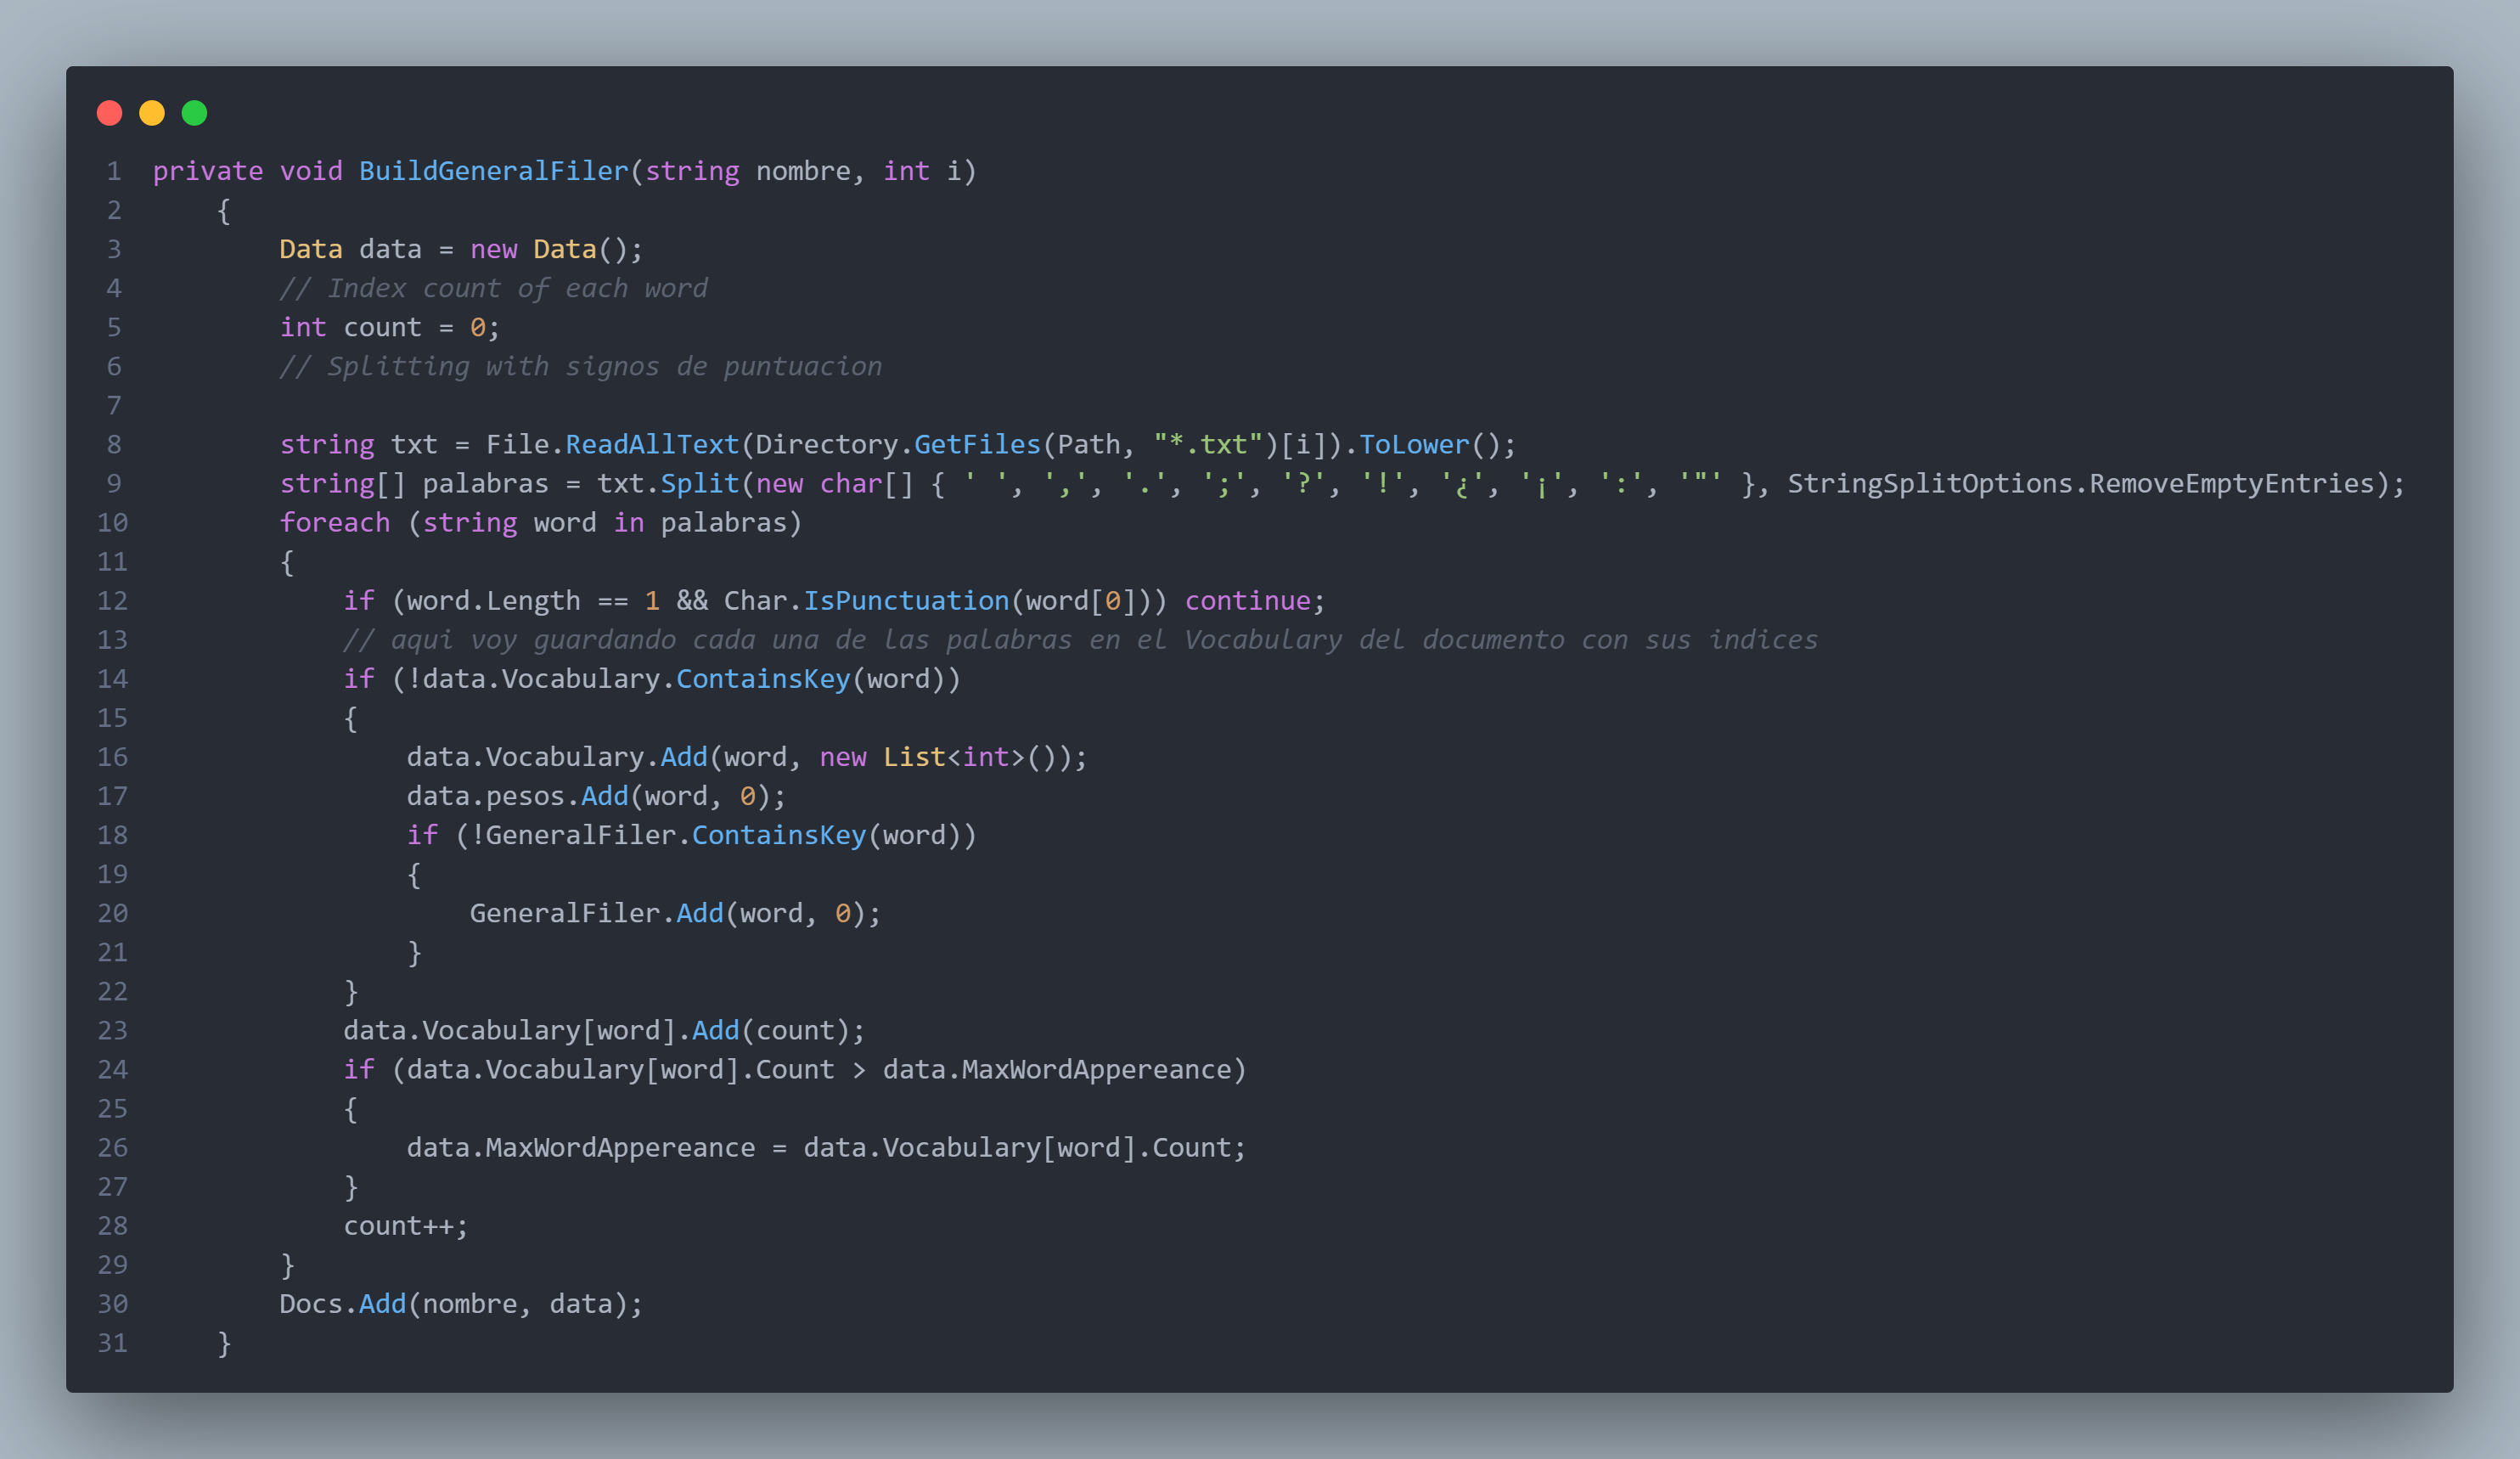
\includegraphics[width=470px]{Assets/Build_General_Filer.png}
                %\caption{Constructor maestro}
            \end{figure}[h]
            \newpage
            \item 3.3.2 Como se puede ver, aquí ocurre casi toda la "magia", aquí se usan métodos propios de los diccionarios como "ContainsKey", "Add", etc. Aqui se va a separar el texto de cada documento por espacios y diferentes caracteres(como se observa arriba), y se va a ir almacenando cada palabra resultante en el vocabulario con sus indices, y finalmente se va a formar el Diccionario docs, con los nombres de los documentos y sus datos
            \begin{itemize}
                \item 2.3.2.1 Estos datos se van recopilando a lo largo del bucle foreach dentro de esta funcion BuildGeneralFiler
            \end{itemize}

            \item 3.4 Data, la clase que contiene los datos de cada documento donde se calcula el peso de cada palabra en el documento que esté analizando en dicho momento, además le da valor a la variable "Module" del documento, que no es mas que el módulo del vector de peso
            
            \item \begin{figure}[h]
                    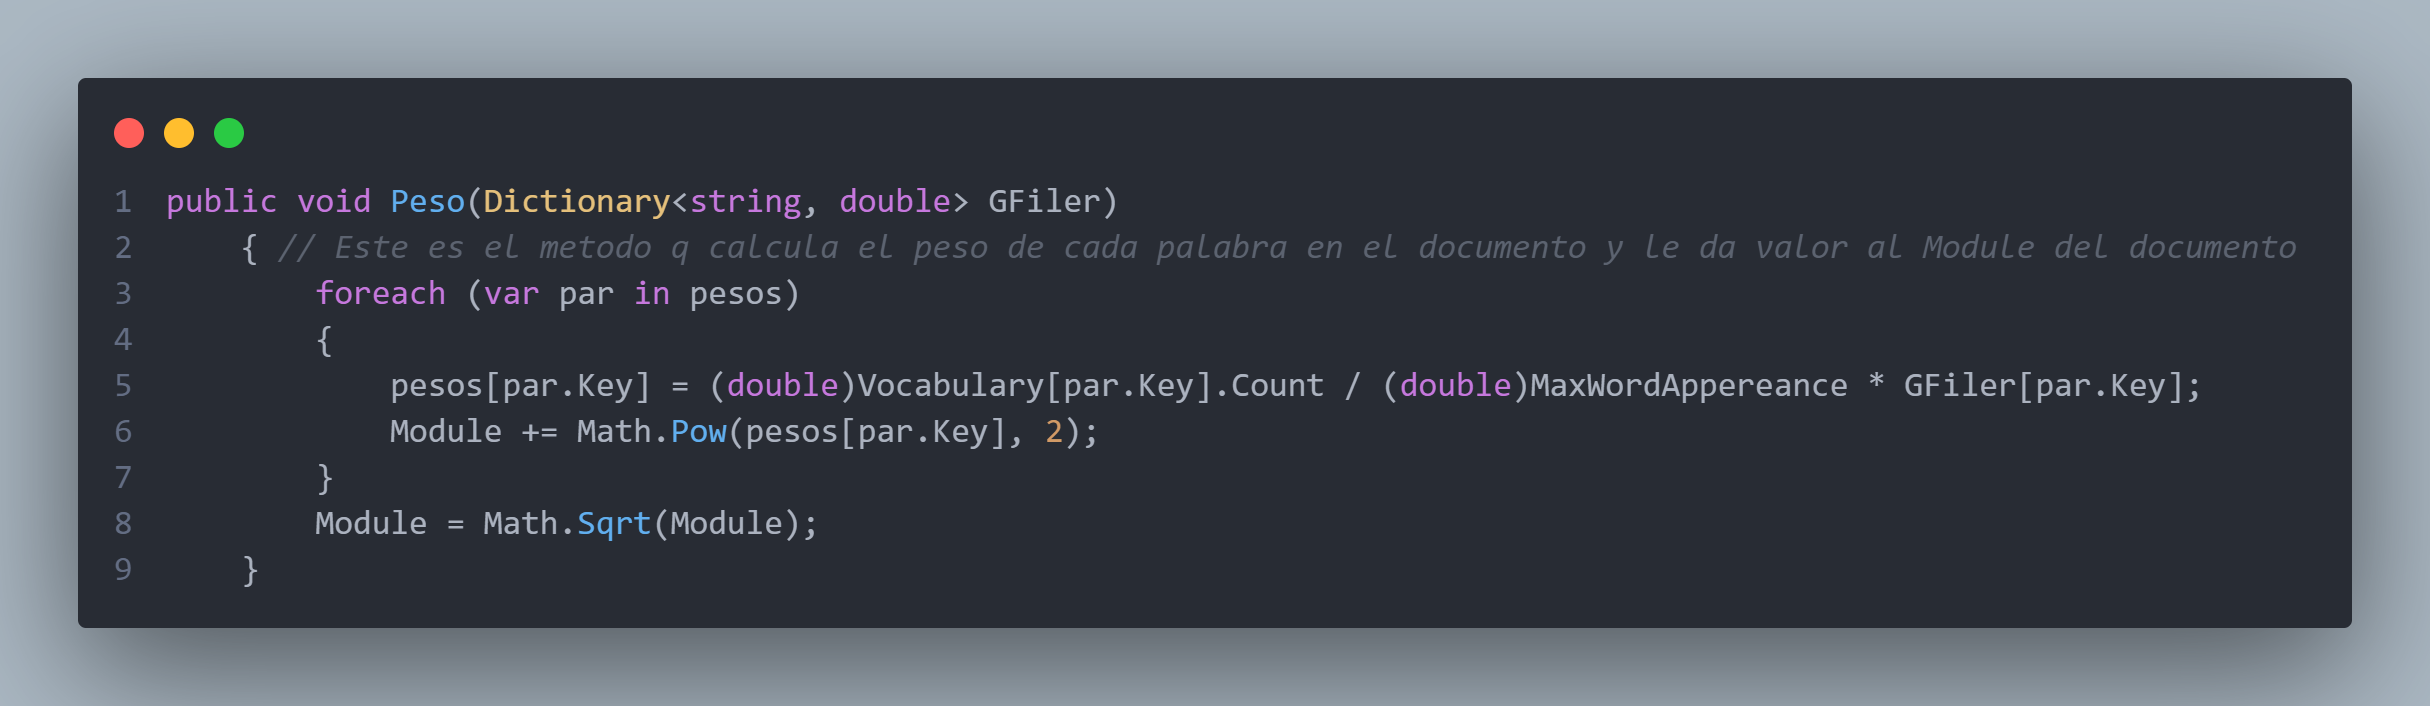
\includegraphics[width=470px]{Assets/Peso.png}
                  \end{figure}
            3.4.1 Otros valores da Data
            int MaxWordAppereance = 0; -> Frecuencia de la palabra que más aparece
            Dictionary Vocabulary -> Este es el vocabulario del documento contra los indices de las palabras de ese vocabulario
        \end{itemize}
    \newpage
    \item MASE: Consulta(Searcher) y Puntaje(Score)
        \begin{itemize}
            \item 4.1 El constructor de la clase, recibe la entrada del usuario(Query) desde el apartado grafico, y un Corpus(El ya creado anteriormente y creado al inicio del proyecto)
                \begin{itemize}
                    \item UsrInp es la consulta del usuario ya procesada, por el metodo ProcessQuery, que lo que hace no es más que separar en terminos la consulta
                    \item LetMeIn(Lista de Inclusion), LetMeOut(Lista de Exclusion), Closeness(Lista de cercanía), se encargaran de recibir los terminos de la búsqueda según los operadores colocados.
                    \item GetInfo, es la función casi que más caótica, aquí primeramente se separan los terminos segun sus operadores, posteriormente cada palabra de la consulta va para el diccionario Frqhzy con su cantidad de repeticiones:
                \end{itemize}
            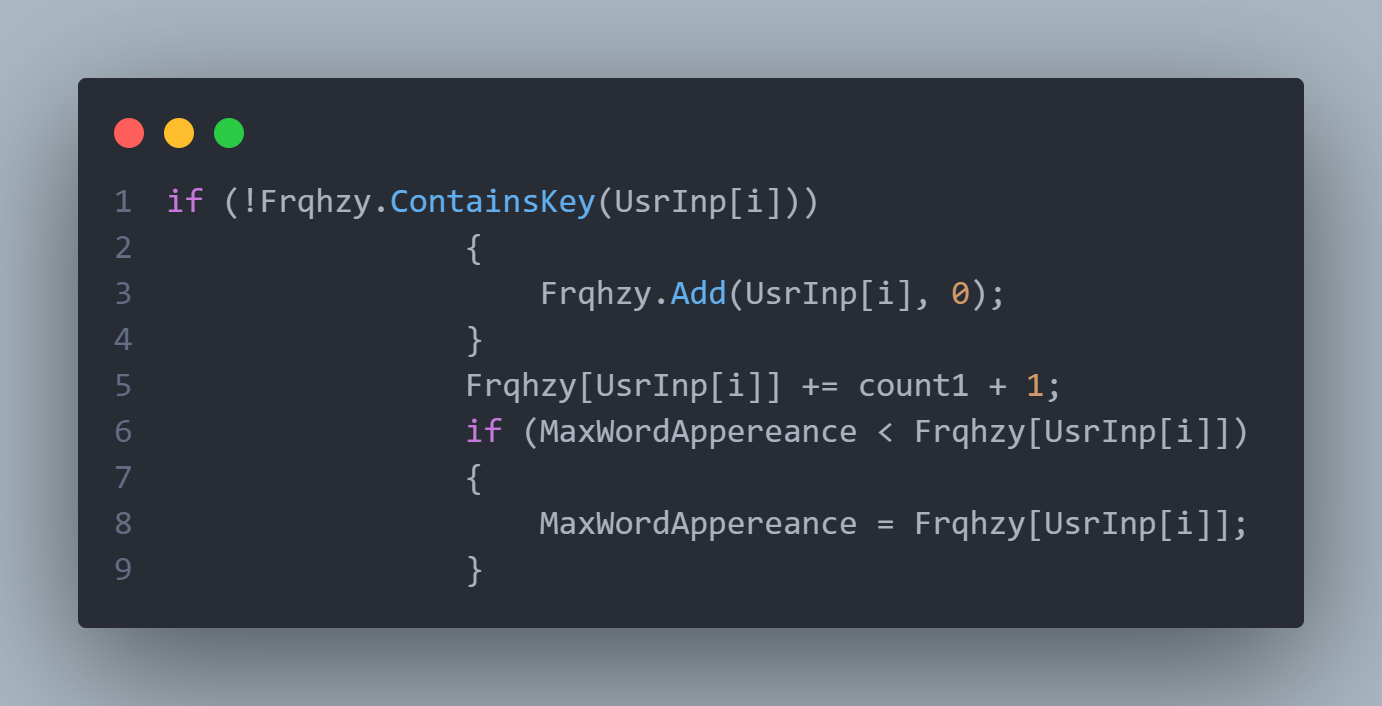
\includegraphics[width=420px]{Assets/frqhzy.png}
            \item 4.2
                \begin{itemize}
                    \item Luego en la linea 43, el corpus declarado en esta clase searcher, pasa a ser el corpus enviado a consultar
                    \item GSuggest, funcion que usando la distancia de Levensthein(Aun no optimizada), sustituye las palabras mal escritas o no encontradas de la consulta, por otras posiblemente más adecuadas. Además incorpora el método Suggestion() 
                    
                \end{itemize}
            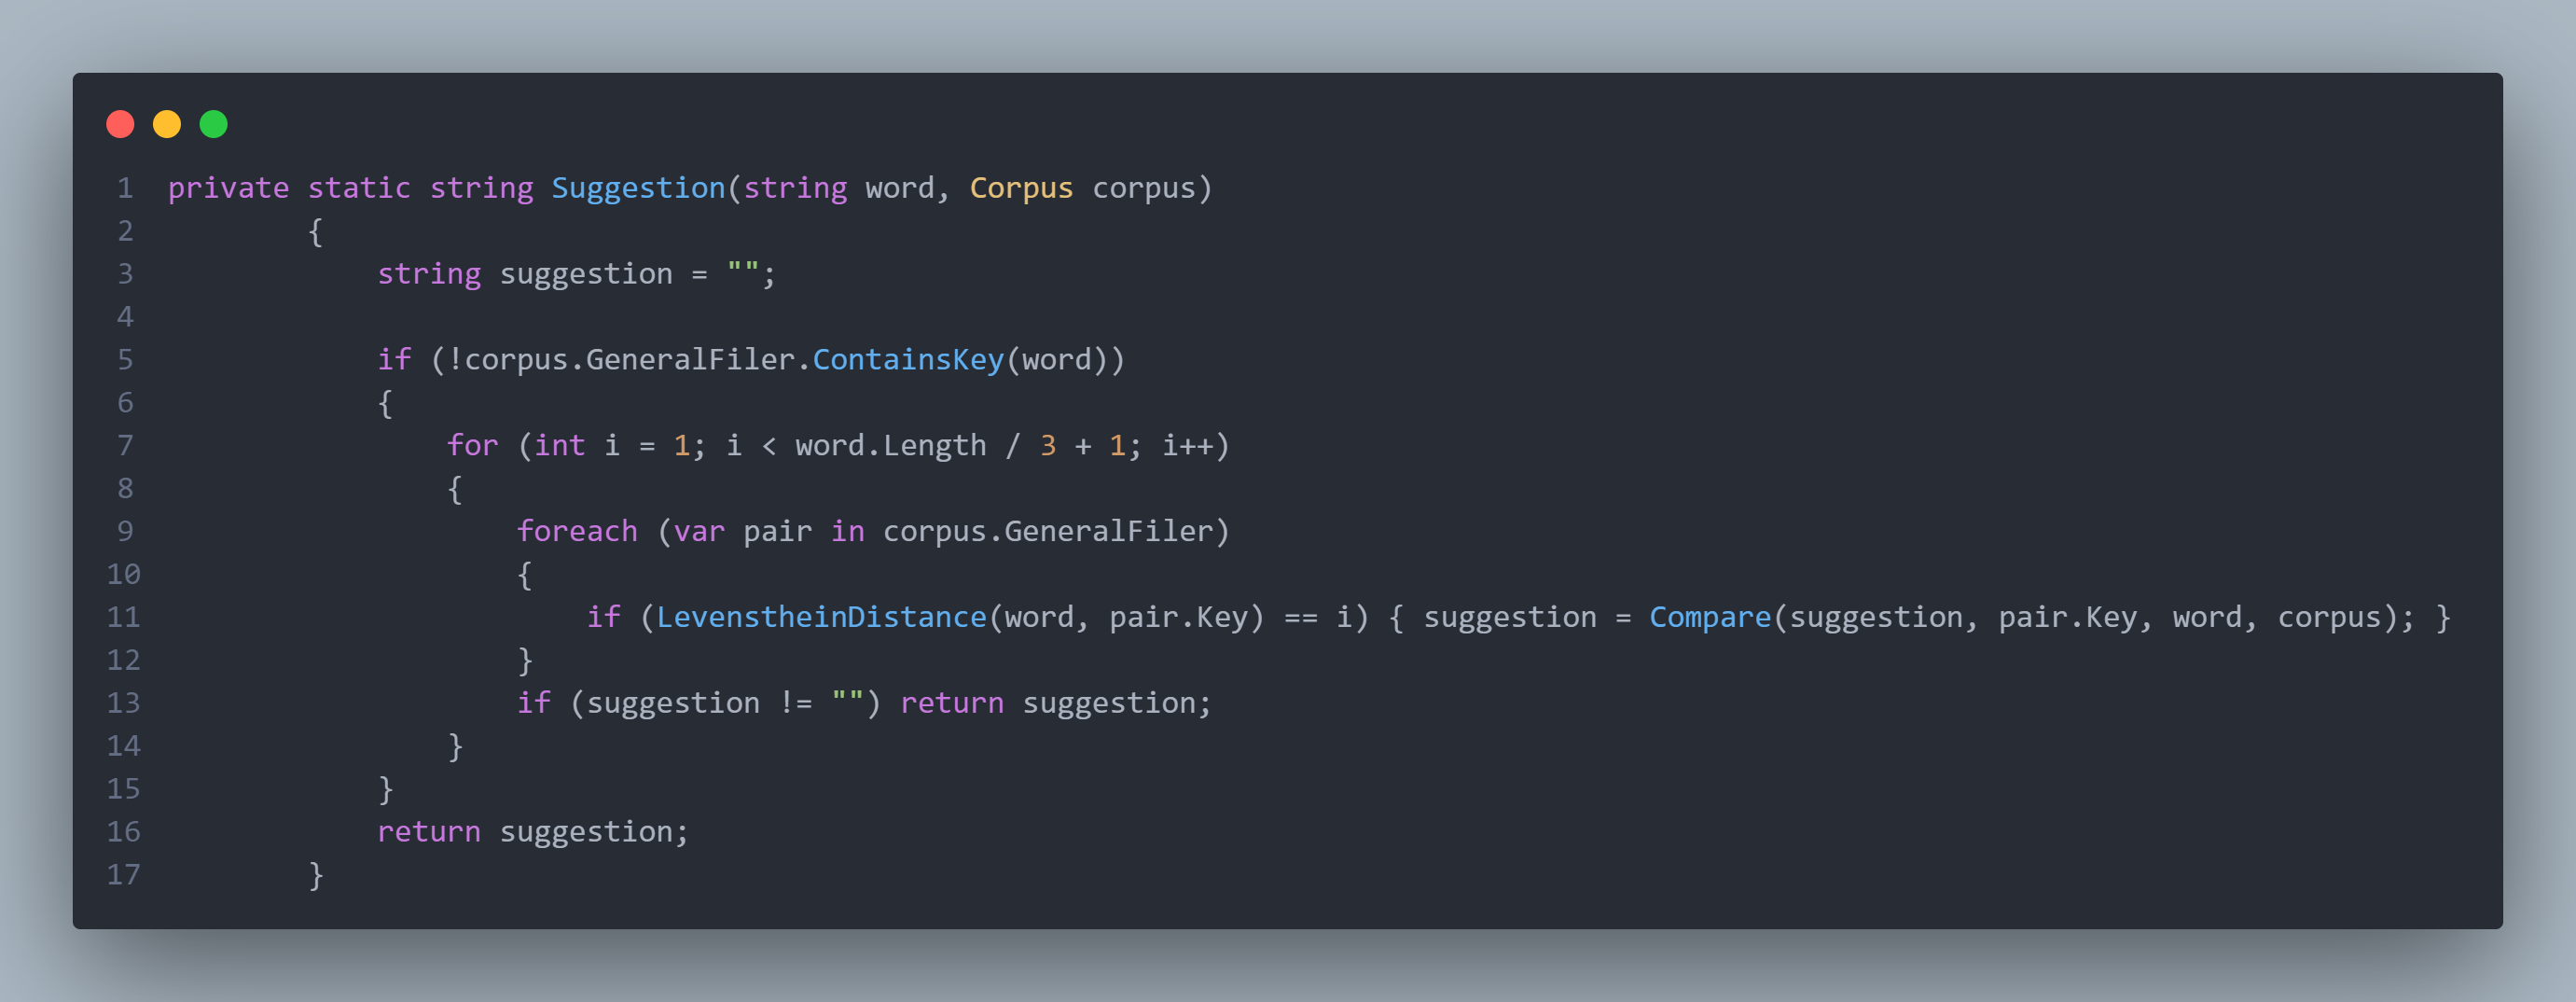
\includegraphics[width=420px]{Assets/Suggestion.png}
                
            \newpage
            \begin{itemize}
                \item Usando la distancia de Levensthein(No optimizada aún), recorre palabra por palabra, para buscar por poca diferencia, la palabra más semejante de la consulta, para finalmente devolverla. [Mi idea es crear al inicio un diccionario extra, o varios, que abarquen todo el Vocabualrio de mis Docs y ordene por tamaño todas las palabras, asó a la hora de sugerir una palabra solo tendría que calcular con palabras 1 caracter más o menos grande, o de igual tamaño]
                \item Snippets = new string[corpus.Docs.Count] crea el string Snippets con longitud igual a la cantidad de documentos, este string pues almacenará eso, los snippets con score != 0.
                \item WVal = new double[UsrInp.Length] es un array de dobles, que tendrá los valores de los terminos de la consulta, con capacidad == cantidad de terminos del UsrInp(Consulta).
                \item 'Save W Value' usando la conocida formula de TF*IDF, pues calcula los valores de peso de los terminos de la consulta. MASE LN -> 57
                \item Mod() Calculará el vector de pesos de la consulta
                
                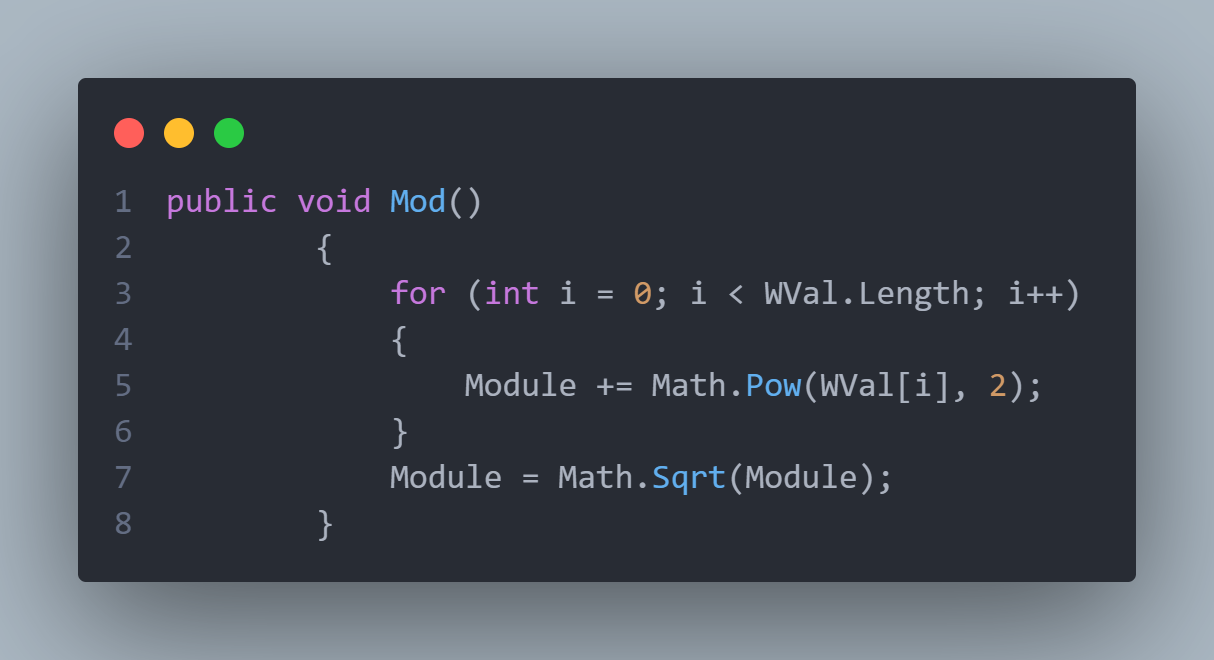
\includegraphics[width=400px]{Assets/Mod.png}

                \item FillSuggest() Metodo que modifica la sugerencia a devolver.
            \end{itemize}
        \end{itemize}
    \item Score:
        \begin{itemize}
            \item 5.1 Clase que guardará los puntajes de cada documento, para finalmente ser mostrado en el partado gráfico
            \begin{itemize}
                \item public Searcher searcher Se declara una consulta
                \item public Corpus Corpus Se declara un corpus
                \item public (string, double)[] tupla Se declara este array que será de igual tamaño que la cantidad de documentos, ademas almacena sus puntajes.
            \end{itemize}
            \newpage
            \item 5.2 El constructor de esta clase
            \begin{itemize}
                \item Comienza recibiendo y tomando una consulta y un corpus
                \item Como había dicho, la tupla se crea, con igual longitud que la cantidad de documentos
                \item FillScores() función que ordena las tuplas de mayor a menor, luego de haber ejecutado un producto vectorial con la funcion VecMultiply:
                
                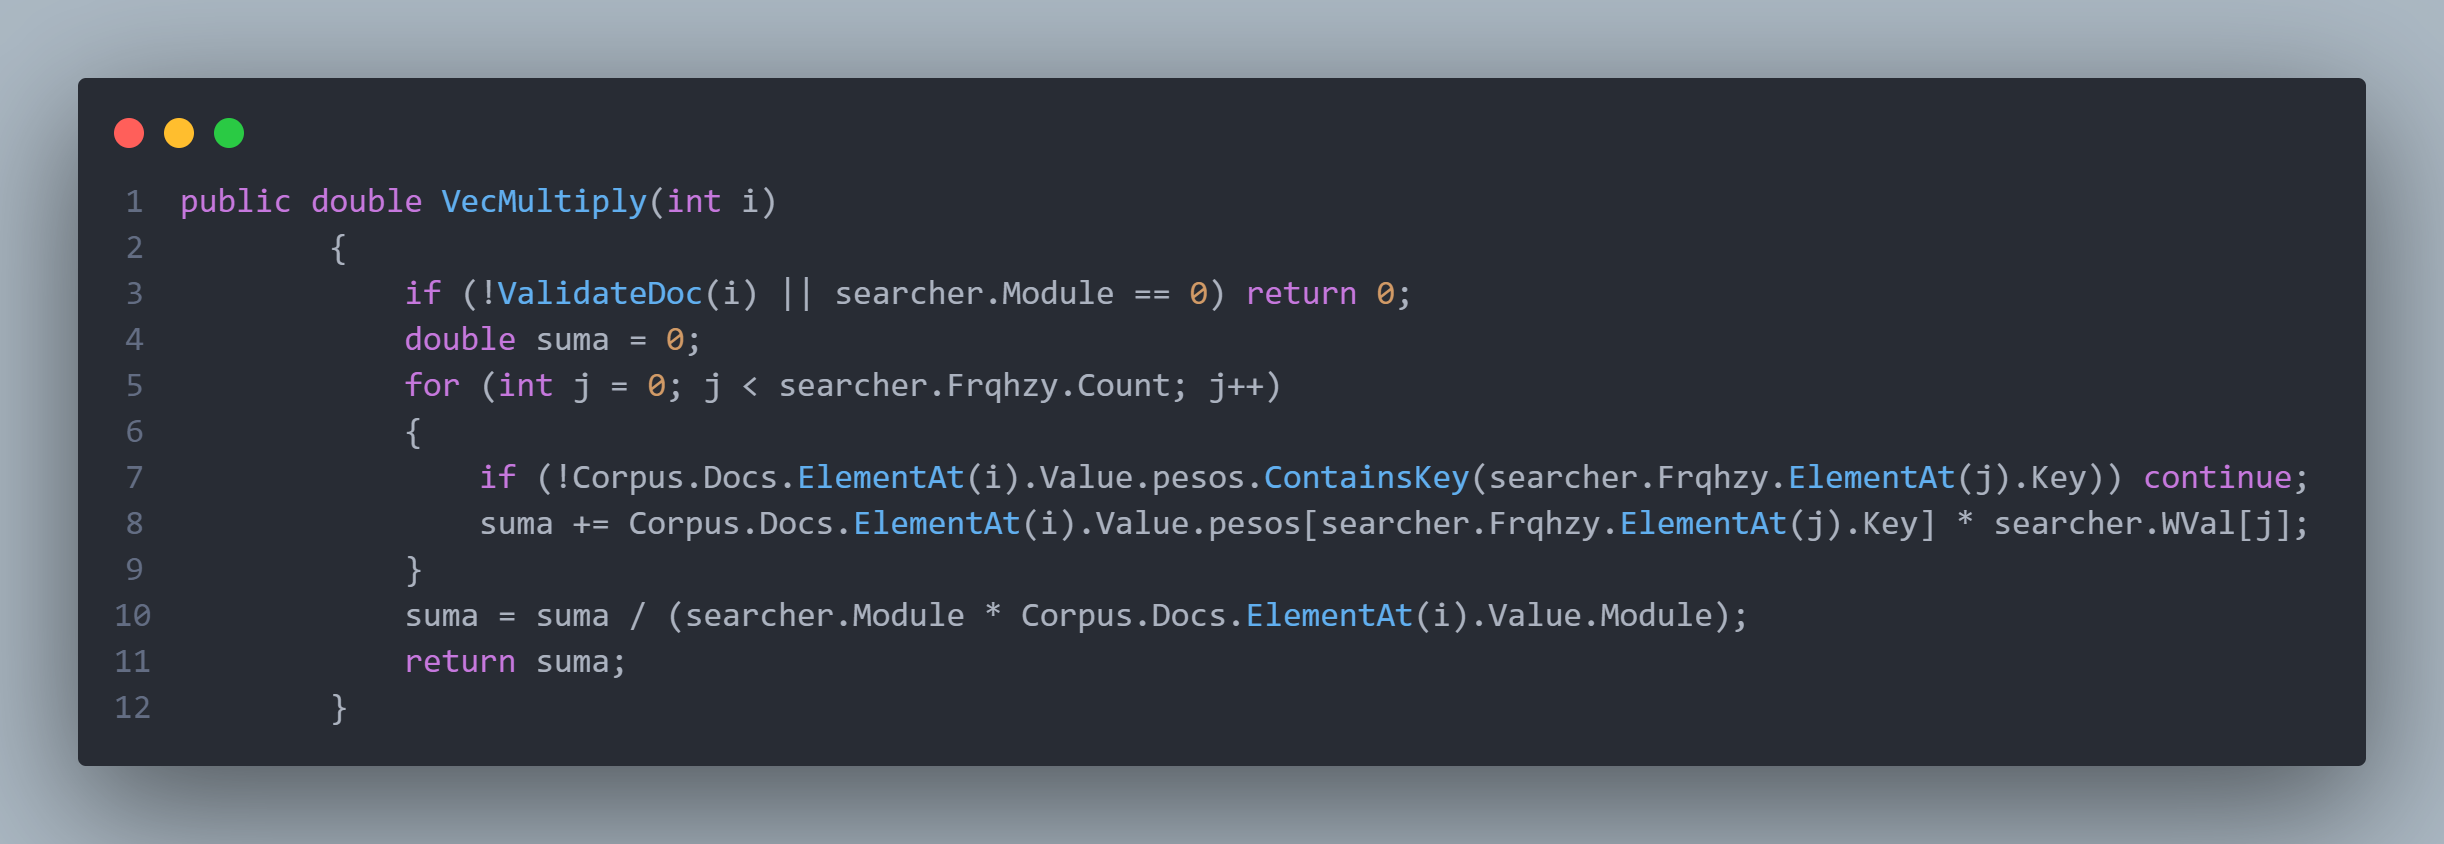
\includegraphics[width=400px]{Assets/VecMultiply.png}

                \item Esta funcion de FillScores(), tambien da inicio a la función FillSnippet(tupla) que va rellenando los snippet(Ver más adelante en la sección 5), además usa un metodo para modifcar el score, llamada ModScore(), que depende de si alguna(s) palabra(s), perteneces a la lista de Closeness y por tanto cambia el score en dependencia de la cercania entre esos terminos. Además usa un BubbleSort(), el metodo de sorteo más sencillo, recorre los terminos a pares y los intercambia si estan en el lugar equivocado.
                \item El metodo ModScore() usa además la función LowestDistance, que como su nombre indica devuelve la menor distancia entre dos términos en un documento.
            \end{itemize}
            \item 5.3
                \begin{itemize}
                    \item Swap() Simple funcion que cambia dos elementos de lugar en un array.
                    \item TotalWeight() Metodo que suma y devuelve los pesos de una palabra en cada aparicion de esta en cada documento. Se usa en la funcion Compare().
                    \item ValidateDoc() Funcion que otorgará puntaje igual a 0 a aquellos documentos que contengan una palabra exluida y tambien otorgará 0 a cada documento que no contenga a una palabra incluida.
                    \item Compare() metodo presente en la clase Searcher, Ln -> 199, que se encargará de devolver entre dos palabras, la más importante usando el método TotalWeight()
                \end{itemize}
        \end{itemize}
    \item Snippet
        \begin{itemize}
            \item 6.1 FillSnippet() es la función, que se encarga de llenar los snippets de aquellos documentos que pasaron el Score(!=0)
            \begin{itemize}
                \item Usa el hilo "Relevant" sinónimo de MASIMPORTANTE, que contendrá la palabra con la cual se presentará el Snippet más adelante.
                \item Al final de la función se invoca el método RetSnippet().
            \end{itemize}
            \item 6.2 RetSnippet() Esta recibirá, esa palabra "Relevant" y el documento donde se encuentre y creará un snippet que contenga esa palabra.
        \end{itemize}
        \newpage
    \item Cambios en SearchItem y SearchResult
        \begin{itemize}
            \item 7.1 SearchItem Score, lo cambié de float a double.
            \item 7.2 SearchResult
            \begin{itemize}
                \item No declaro un objeto SearchItem[], sino una List<SearchItem> items, del mismo nombre.
                \item El constructor de esta clase ahora recibe List<SearchItem> items, y su sobrecarga ahora hereda una Lista igualmente.
                \item La variable "Count" devuelve this.items.Count en lugar de this.items.Length
            \end{itemize}
        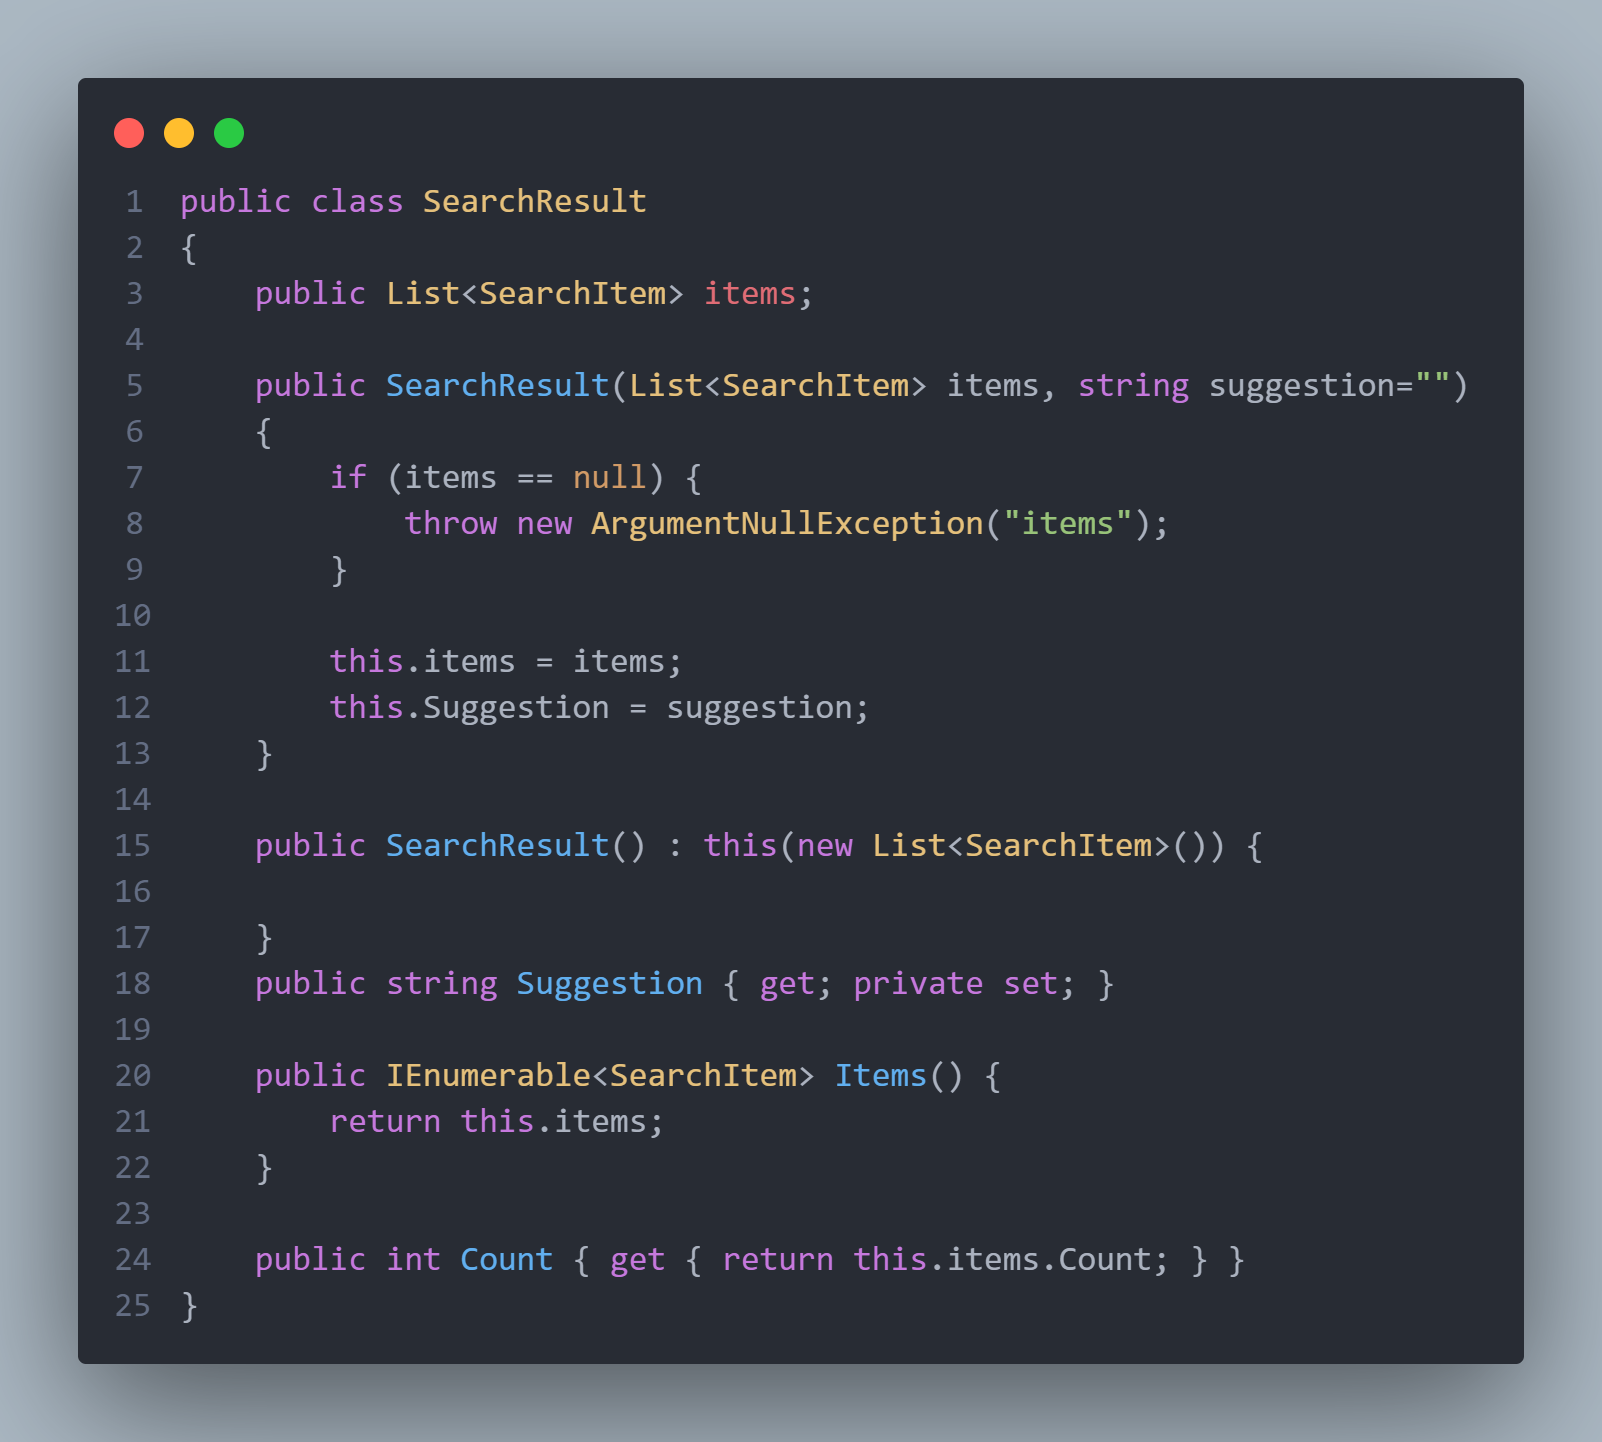
\includegraphics[width=420px]{Assets/SearchResult.png}
        \end{itemize}
        \newpage
    \item Retornando al inicio:
        \begin{itemize}
            \item 8.1 La clase Moogle ahora:
                \begin{itemize}
                    \item Declara un Corpus, el mismo que da inicio al programa, y el cual se usará para la búsqueda.
                    \item Declara una Consulta(searcher), la cual hará todos los pasos y metodos anteriormente explicados.
                    \item Declara un Score, puntaje que una vez procesado, será mostrado en pantalla, una vez culmine la búsqueda
                    \item Un cronómetro(No Funcional... por ahora) que mostrará cuanto tardó la consulta (Google-like)
                    \item Finalmente método "Query" de tipo SearchResult
                    \begin{itemize}
                        \item Dará orden de inicio a Searcher
                        \item Dará orden de inicio a Score
                    \end{itemize}
                    \item Esta función "Query" devolverá los "items"(Titulo, Snippet, Score) y la sugerencia final.
                \end{itemize}
            \item 8.2 En Index.razor:
                \begin{itemize}
                    \item Existe una nueva variable double que tendrá el valor en segundos del tiempo tomado en procesar la consulta.
                    \item A esta región le agregué el "Score".
                    
                    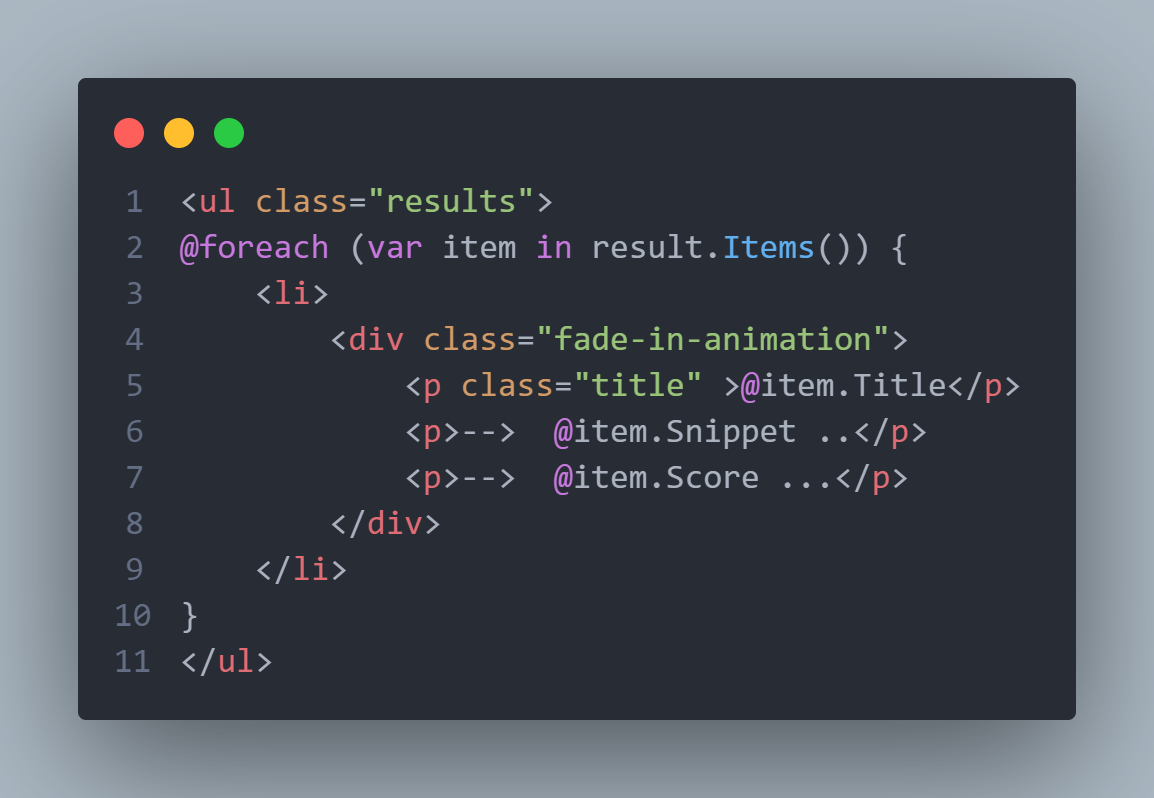
\includegraphics[width=400px]{Assets/IndexRazor.png}
                    
                    %\item Debajo de la sugerencia irá el tiempo tomado. (Se me ocurrió a ultima hora).
                \end{itemize}
        \end{itemize}
    \item The End
\end{enumerate}

\end{document}